\documentclass{article}
\usepackage{graphicx}
\usepackage{subcaption}

\usepackage{geometry}

% Set custom page margins
\geometry{
  left=1cm,
  right=1cm,
  top=1cm,
  bottom=1cm
}

\begin{document}

\begin{figure}[ht]
    \centering
    % Large top image
    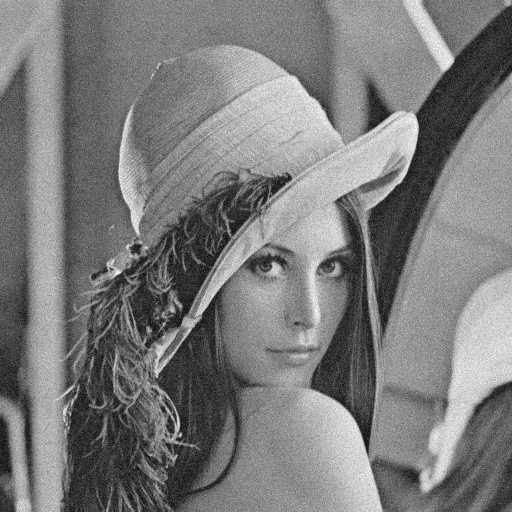
\includegraphics[width=0.3\textwidth]{gn10.png}
    \caption{gaussian noise 10}
    \label{fig:top_image}

    % First row of smaller images
    \begin{subfigure}{0.3\textwidth}
        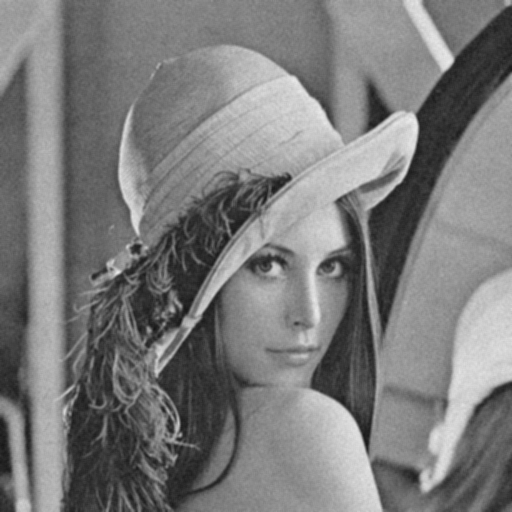
\includegraphics[width=\linewidth]{gn10_b3.png}
        \caption{box $3 \times 3$}
        \label{fig:sub1}
    \end{subfigure}
    \begin{subfigure}{0.3\textwidth}
        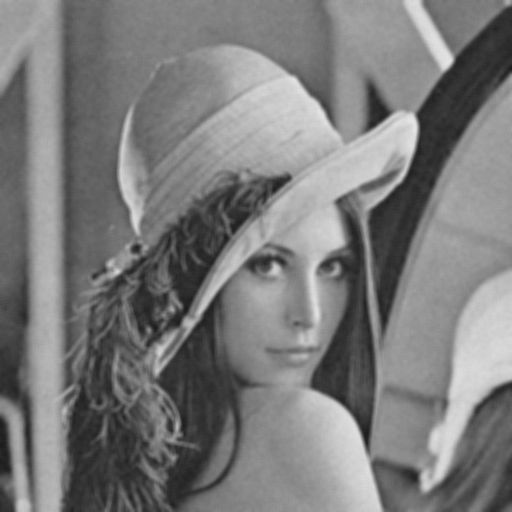
\includegraphics[width=\linewidth]{gn10_b5.png}
        \caption{box $5 \times 5$}
        \label{fig:sub2}
    \end{subfigure}

    % Second row of smaller images
    \begin{subfigure}{0.3\textwidth}
        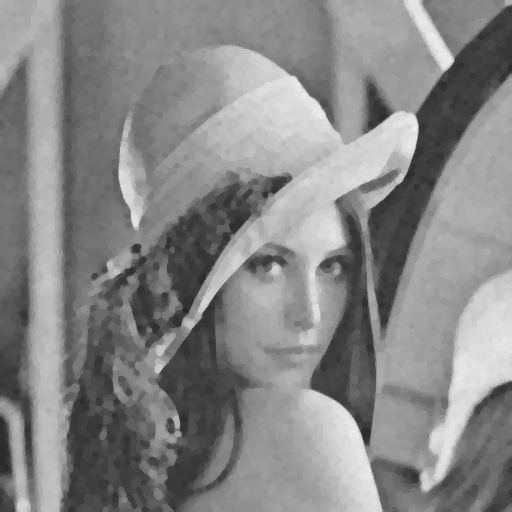
\includegraphics[width=\linewidth]{gn10_cto.png}
        \caption{close then open}
        \label{fig:sub3}
    \end{subfigure}%
    \begin{subfigure}{0.3\textwidth}
        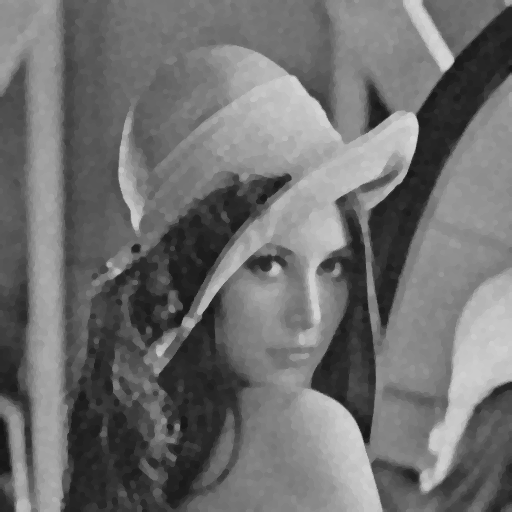
\includegraphics[width=\linewidth]{gn10_otc.png}
        \caption{open then close}
        \label{fig:sub4}
    \end{subfigure}

    % Third row of smaller images
    \begin{subfigure}{0.3\textwidth}
        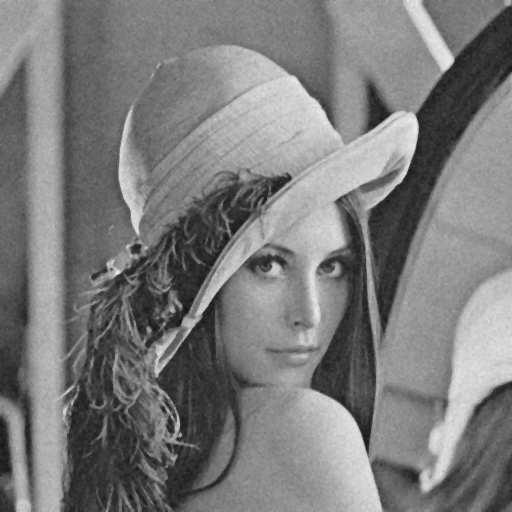
\includegraphics[width=\linewidth]{gn10_m3.png}
        \caption{median $3 \times 3$}
        \label{fig:sub5}
    \end{subfigure}%
    \begin{subfigure}{0.3\textwidth}
        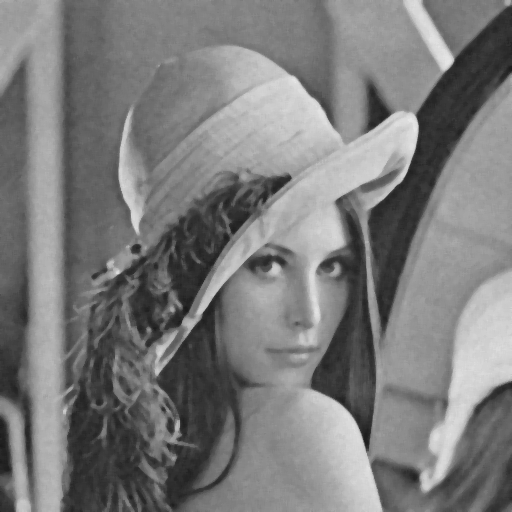
\includegraphics[width=\linewidth]{gn10_m5.png}
        \caption{median $5 \times 5$}
        \label{fig:sub6}
    \end{subfigure}

\end{figure}
\newpage
\begin{figure}[ht]
    \centering
    % Large top image
    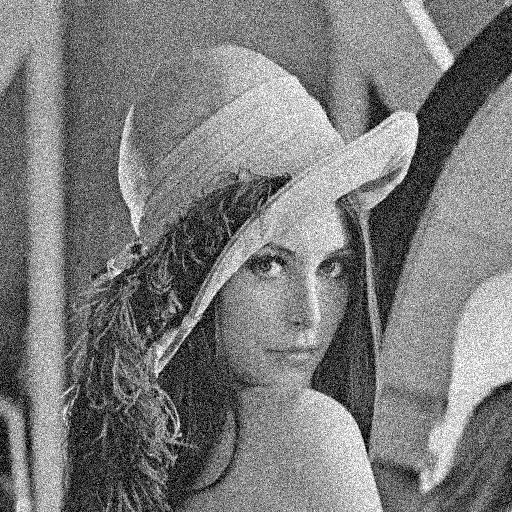
\includegraphics[width=0.3\textwidth]{gn30.png}
    \caption{gaussian noise 30}
    \label{fig:top_image}

    % First row of smaller images
    \begin{subfigure}{0.3\textwidth}
        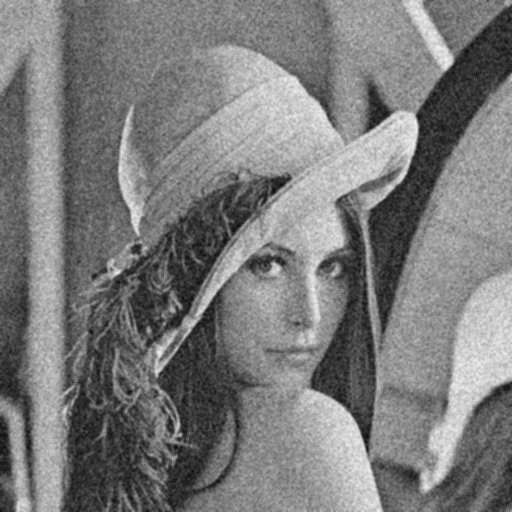
\includegraphics[width=\linewidth]{gn30_b3.png}
        \caption{box $3 \times 3$}
        \label{fig:sub1}
    \end{subfigure}
    \begin{subfigure}{0.3\textwidth}
        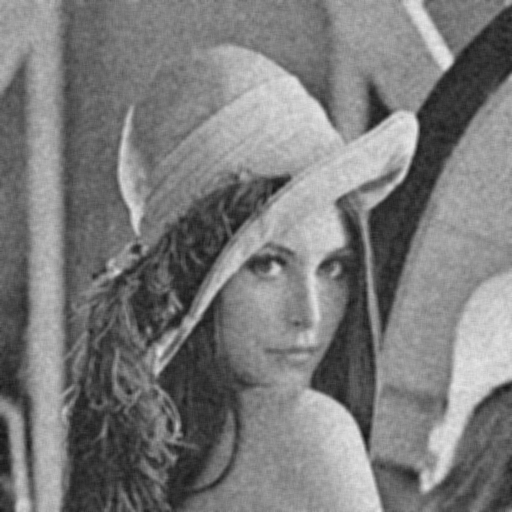
\includegraphics[width=\linewidth]{gn30_b5.png}
        \caption{box $5 \times 5$}
        \label{fig:sub2}
    \end{subfigure}

    % Second row of smaller images
    \begin{subfigure}{0.3\textwidth}
        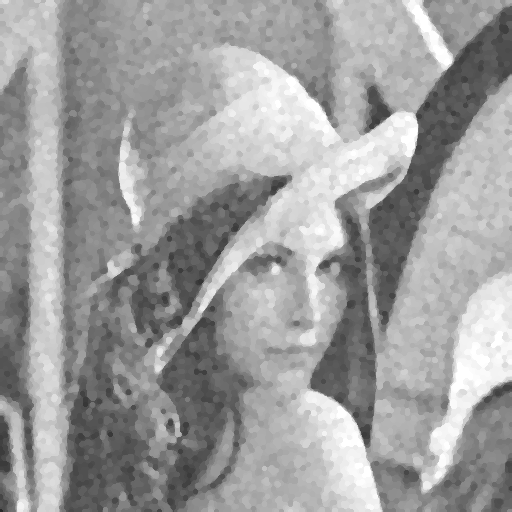
\includegraphics[width=\linewidth]{gn30_cto.png}
        \caption{close then open}
        \label{fig:sub3}
    \end{subfigure}%
    \begin{subfigure}{0.3\textwidth}
        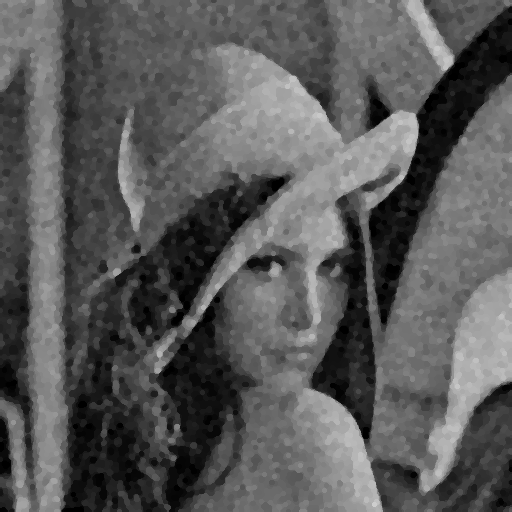
\includegraphics[width=\linewidth]{gn30_otc.png}
        \caption{open then close}
        \label{fig:sub4}
    \end{subfigure}

    % Third row of smaller images
    \begin{subfigure}{0.3\textwidth}
        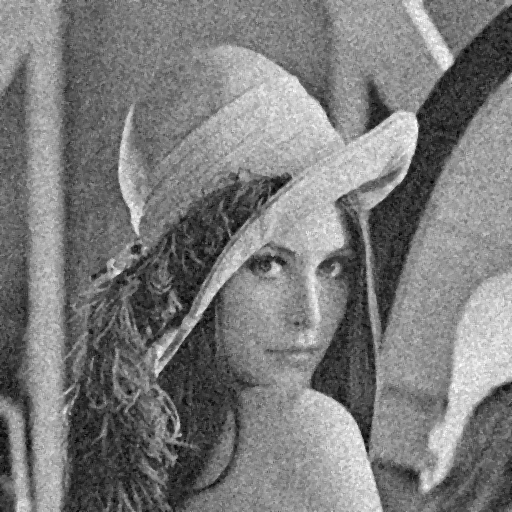
\includegraphics[width=\linewidth]{gn30_m3.png}
        \caption{median $3 \times 3$}
        \label{fig:sub5}
    \end{subfigure}%
    \begin{subfigure}{0.3\textwidth}
        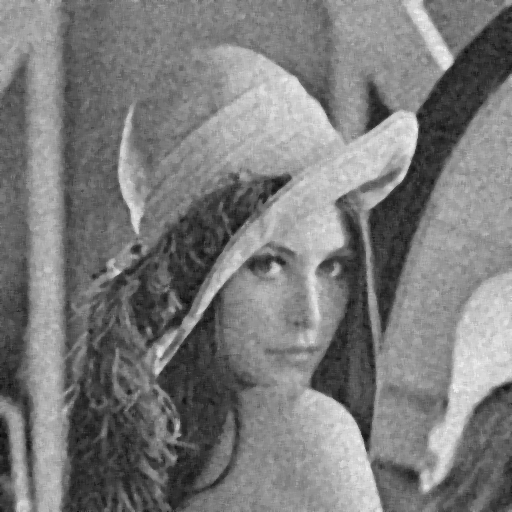
\includegraphics[width=\linewidth]{gn30_m5.png}
        \caption{median $5 \times 5$}
        \label{fig:sub6}
    \end{subfigure}

\end{figure}
\newpage
\begin{figure}[ht]
    \centering
    % Large top image
    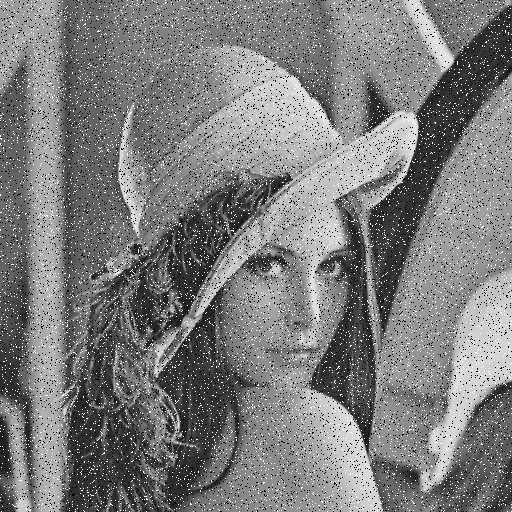
\includegraphics[width=0.3\textwidth]{sp05.png}
    \caption{salt and pepper 0.05}
    \label{fig:top_image}

    % First row of smaller images
    \begin{subfigure}{0.3\textwidth}
        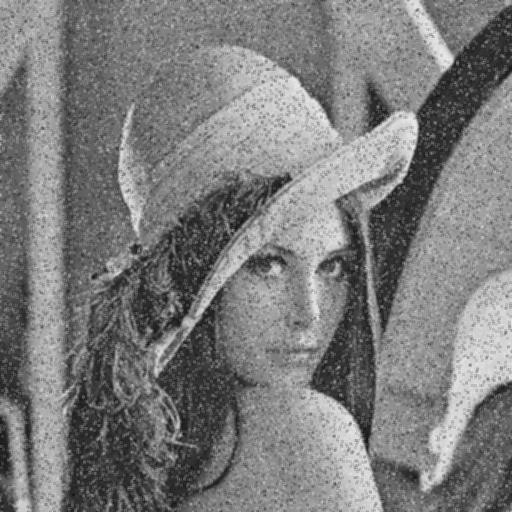
\includegraphics[width=\linewidth]{sp05_b3.png}
        \caption{box $3 \times 3$}
        \label{fig:sub1}
    \end{subfigure}
    \begin{subfigure}{0.3\textwidth}
        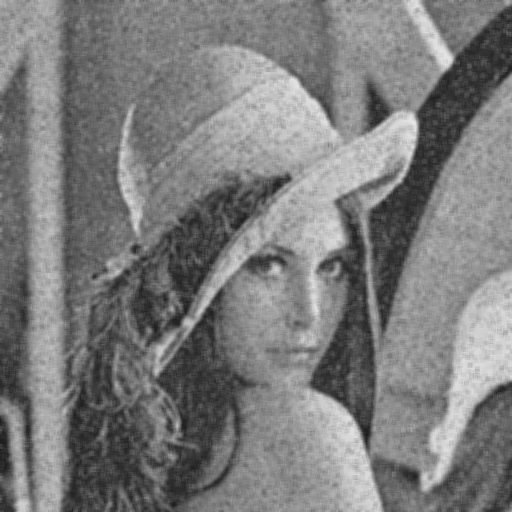
\includegraphics[width=\linewidth]{sp05_b5.png}
        \caption{box $5 \times 5$}
        \label{fig:sub2}
    \end{subfigure}

    % Second row of smaller images
    \begin{subfigure}{0.3\textwidth}
        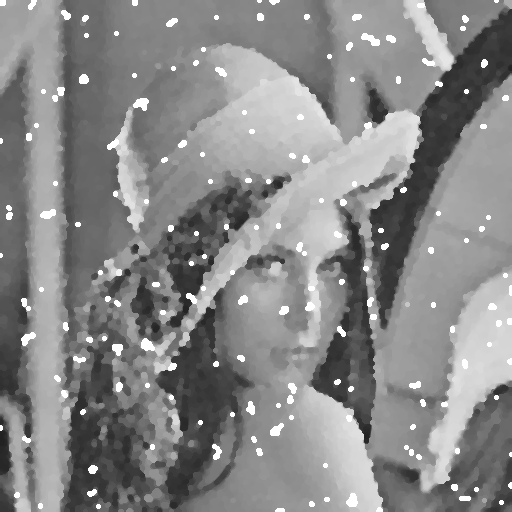
\includegraphics[width=\linewidth]{sp05_cto.png}
        \caption{close then open}
        \label{fig:sub3}
    \end{subfigure}%
    \begin{subfigure}{0.3\textwidth}
        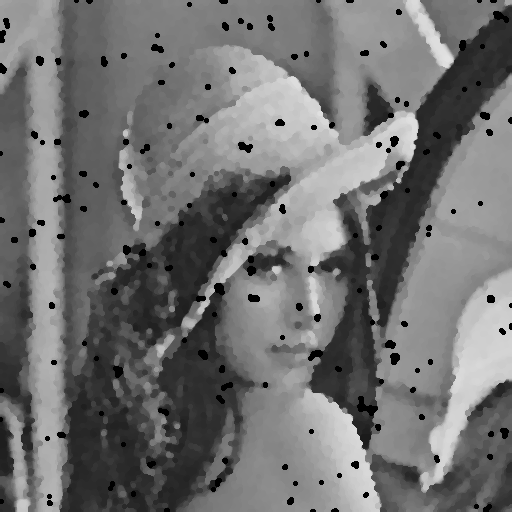
\includegraphics[width=\linewidth]{sp05_otc.png}
        \caption{open then close}
        \label{fig:sub4}
    \end{subfigure}

    % Third row of smaller images
    \begin{subfigure}{0.3\textwidth}
        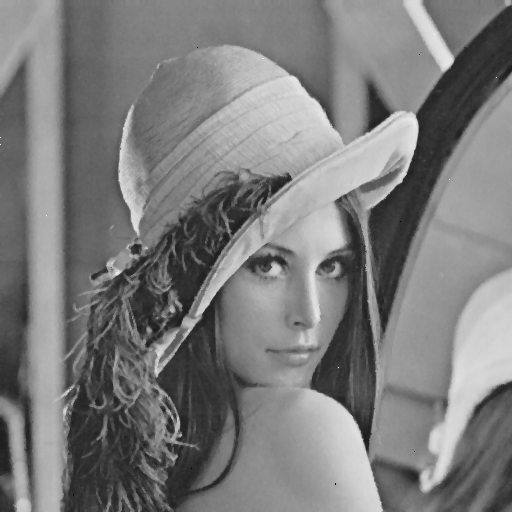
\includegraphics[width=\linewidth]{sp05_m3.png}
        \caption{median $3 \times 3$}
        \label{fig:sub5}
    \end{subfigure}%
    \begin{subfigure}{0.3\textwidth}
        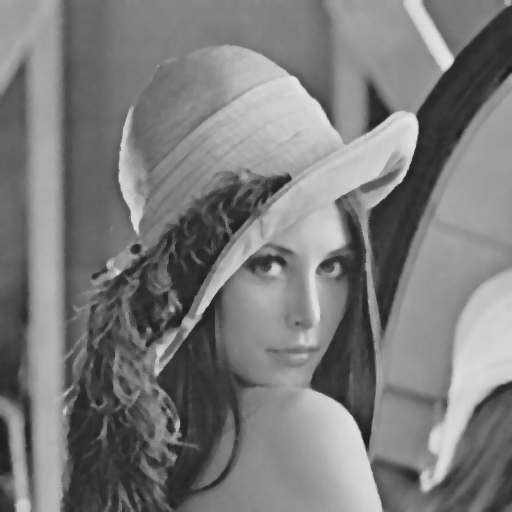
\includegraphics[width=\linewidth]{sp05_m5.png}
        \caption{median $5 \times 5$}
        \label{fig:sub6}
    \end{subfigure}

\end{figure}
\newpage
\begin{figure}[ht]
    \centering
    % Large top image
    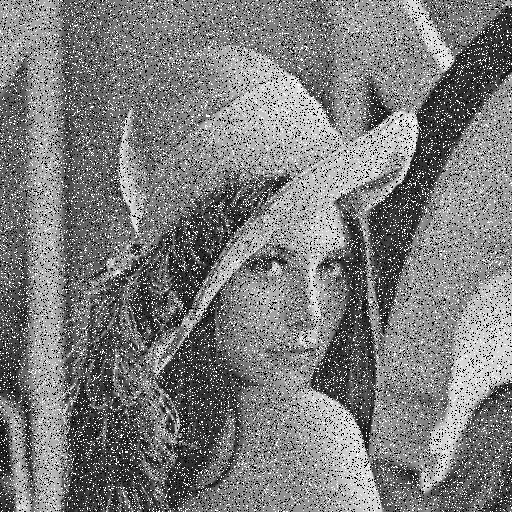
\includegraphics[width=0.3\textwidth]{sp10.png}
    \caption{salt and pepper 0.10}
    \label{fig:top_image}

    % First row of smaller images
    \begin{subfigure}{0.3\textwidth}
        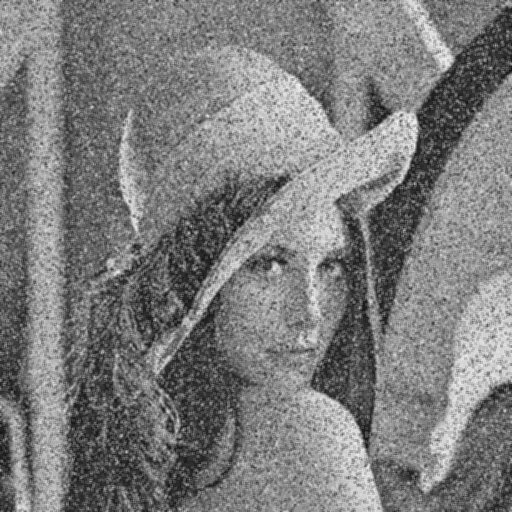
\includegraphics[width=\linewidth]{sp10_b3.png}
        \caption{box $3 \times 3$}
        \label{fig:sub1}
    \end{subfigure}
    \begin{subfigure}{0.3\textwidth}
        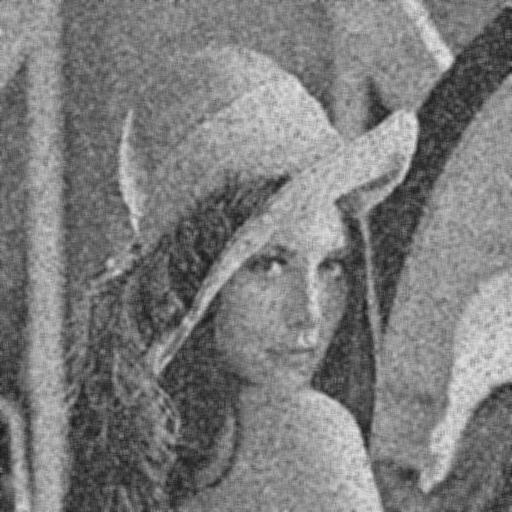
\includegraphics[width=\linewidth]{sp10_b5.png}
        \caption{box $5 \times 5$}
        \label{fig:sub2}
    \end{subfigure}

    % Second row of smaller images
    \begin{subfigure}{0.3\textwidth}
        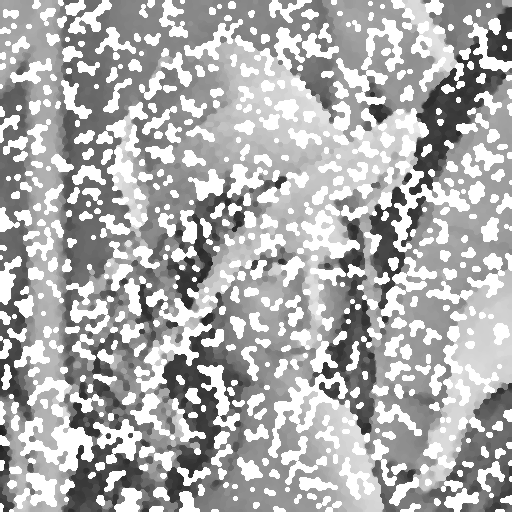
\includegraphics[width=\linewidth]{sp10_cto.png}
        \caption{close then open}
        \label{fig:sub3}
    \end{subfigure}%
    \begin{subfigure}{0.3\textwidth}
        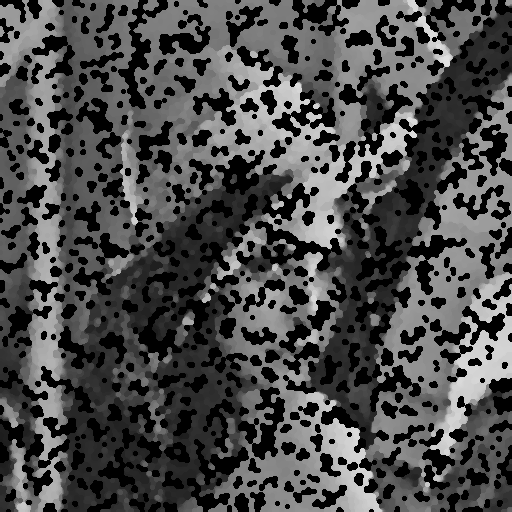
\includegraphics[width=\linewidth]{sp10_otc.png}
        \caption{open then close}
        \label{fig:sub4}
    \end{subfigure}

    % Third row of smaller images
    \begin{subfigure}{0.3\textwidth}
        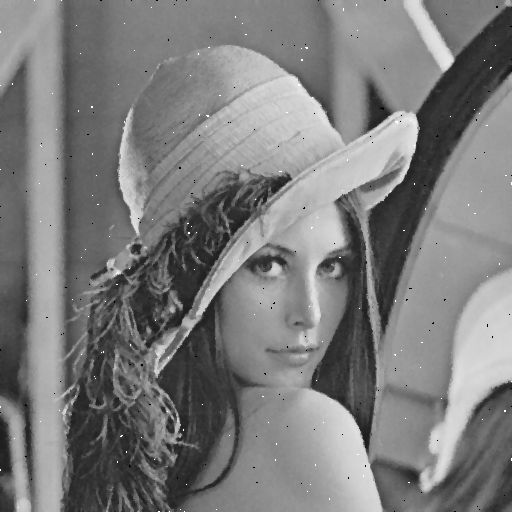
\includegraphics[width=\linewidth]{sp10_m3.png}
        \caption{median $3 \times 3$}
        \label{fig:sub5}
    \end{subfigure}%
    \begin{subfigure}{0.3\textwidth}
        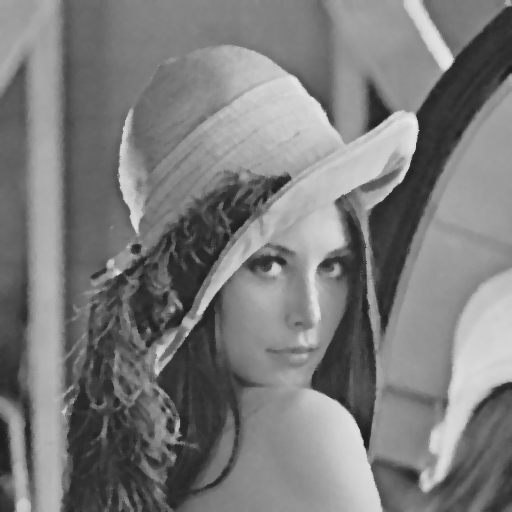
\includegraphics[width=\linewidth]{sp10_m5.png}
        \caption{median $5 \times 5$}
        \label{fig:sub6}
    \end{subfigure}

\end{figure}

\begin{table}[ht]
\centering
\caption{Signal-to-Noise Ratio (SNR) Values for Various Filters}
\begin{tabular}{|l|l|l|}
\hline
\textbf{Image \& Filter} & \textbf{Filter Size} & \textbf{SNR (dB)} \\ \hline

gn10 box & 3 & 17.72585 \\ \hline
gn10 median & 3 & 17.64679 \\ \hline
gn10 box & 5 & 14.85610 \\ \hline
gn10 median & 5 & 15.98067 \\ \hline
gn30 box & 3 & 12.59351 \\ \hline
gn30 median & 3 & 11.06853 \\ \hline
gn30 box & 5 & 13.28099 \\ \hline
gn30 median & 5 & 12.86523 \\ \hline
sp10 box & 3 & 6.310540 \\ \hline
sp10 median & 3 & 15.07231 \\ \hline
sp10 box & 5 & 8.475880 \\ \hline
sp10 median & 5 & 15.79948 \\ \hline
sp05 box & 3 & 9.441888 \\ \hline
sp05 median & 3 & 19.22108 \\ \hline
sp05 box & 5 & 11.13132 \\ \hline
sp05 median & 5 & 16.33672 \\ \hline
gn10 otc & - & 13.19292 \\ \hline
gn10 cto & - & 13.58968 \\ \hline
gn30 otc & - & 11.17649 \\ \hline
gn30 cto & - & 11.20102 \\ \hline
sp10 otc & - & -2.21646 \\ \hline
sp10 cto & - & -2.46925 \\ \hline
sp05 otc & - & 5.551248 \\ \hline
sp05 cto & - & 5.259683 \\ \hline

\end{tabular}
\end{table}


\end{document}

